\documentclass[letterpaper]{article}
\usepackage{amssymb}
\usepackage{fullpage}
\usepackage{amsmath}
\usepackage{epsfig,float,alltt}
\usepackage{psfrag,xr}
\usepackage[T1]{fontenc}
\usepackage{url}
\author{Prof. Grizzle}
\title{Rob 501 - Mathematics for Robotics\\
HW \#3}

\begin{document}
\date{}
\maketitle


 \newcommand{\trace}{\mathrm{trace}}
\newcommand{\real}{\mathbb R}  % real numbers  {I\!\!R}
\newcommand{\nat}{\mathbb N}   % Natural numbers {I\!\!N}
\newcommand{\cp}{\mathbb C}    % complex numbers  {I\!\!\!\!C}
\newcommand{\ds}{\displaystyle}
\newcommand{\mf}[2]{\frac{\ds #1}{\ds #2}}
\newcommand{\Nagy}[2]{{Nagy, Page~#1, }{Prob.~#2}}
\newcommand{\spanof}[1]{\textrm{span} \{ #1 \}}
\parindent 0pt


\begin{flushright}
{\bfseries Due Sept. 27, 2018} \\
{\bfseries 3PM via Gradescope} \\[3mm]
\end{flushright}

\noindent \textbf{Preliminaries:}  Read Chapter 4 of Nagy.


%\noindent \textbf{Terminology:} Any function from a set $S$ to the
%real numbers is often called a functional. ${\rm ker}~f$ is the
%nullspace of $f$. $\spanof {x} = [x]$.

\begin{enumerate}


%Prob. 1 Span
\item \Nagy{117}{4.1.5} (denote the field by $\mathcal{F}$).

%Prob. 2 Linear independence
\item \Nagy{121}{4.2.1}  (the field is $\real$)

%Prob. 3 Linear independence
\item \Nagy{121}{4.2.5} (the field is $\real$) (Note: there is a typo. The last part should be ``show linearly independent OR dependent.'')

%Prob. 4 Span
\item  Let $(X,\mathcal{F})$ be a vector space and $S\subset X$ a subset (not necessarily a subspace).  Prove the following \textbf{Claim:} If $Y$ is a subspace of $X$ and $S \subset Y$, then $\spanof{S} \subset Y$.\\

    \noindent \textbf{Remark:} Usually the result is stated as  ``$\spanof{S}$ is the smallest subspace of $X$ that contains $S$''. The claim is a restatement of this in a form that will make it easier for you to see what needs to be shown.

%Prob. 5 Direct Sums
\item  Let $(X,\mathcal{F})$ be a vector space and $V$ and $W$ subspaces of $X$.  Prove the following \textbf{Claim:} The following two statements are equivalent:
\begin{enumerate}
\setlength{\itemsep}{.1in}
\renewcommand{\labelenumi}{(\alph{enumi})}
\item $V \cap W = \{0\}$

\item For every $x\in V+W$, there exist unique $v\in V$ and $w\in W$ such that $x=v+w$.\\

\noindent \textbf{Remark:} $V+W := \{ v+w~|~ v\in V,~w \in W \}$ and is called the \textit{sum} of $V$ and $W$. When $V \cap W=\{0\}$, one writes $V\oplus W$ and calls it a \textit{direct sum}. The intersection cannot be empty because the zero vector is an element of every subspace!

\end{enumerate}
%Prob. 6 Bases
\item \Nagy{130}{4.3.2}  (the field is $\real$ and the vector space is $\real^4$)

%Prob. 7 Representation of a vector
\item \Nagy{136}{4.4.2}  (the field is $\real$ and the vector space is $\real^3$) Using the vocabulary from lecture, the problem is to find the representation of the vector
    $$ x = \begin{bmatrix} 8 \\ 7 \\4 \end{bmatrix} $$
    in the basis ${\cal U}=\{ u_{1s}, u_{2s}, u_{3s} \}$.

%Prob. 8 Change of basis matrix
\item Using the data in Prob. 7 (that is,  \Nagy{136}{4.4.2}), find the change of basis matrix $P$ from the standard basis $\{ e_1, e_2, e_3 \} $ to the new basis $\{ u_{1s}, u_{2s}, u_{3s} \}$.

%Prob. 9 Change of basis matrix, Rotation Matrix
\item A sensor is mounted on a robot that can turn in place. Figure \ref{robot_ref_frame} shows the robot rotated by an angle $\theta$. Find the change of basis matrix $P$, $([x]_R=P[x]_W )$ from the world reference frame $(X_W, Y_W)$ to the robot's reference frame $(X_R, Y_R)$. 
    
    \noindent \textbf{Remark:} In practice, imagine you have mounted a camera on the robot and observe an object; it will be in the frame of the robot, which moves with the robot. Being able to relate the object's position in a fixed (global or world) reference frame is of obvious interest. In fact, for navigation in driverless cars, one idea being pursued is to provide the car with a 3D enhanced map that will allow the car to tell where it is by what it sees. In our problem, if you know where an object is in the frame of the robot and in the world frame, you can determine the angle $\theta$.
    
\begin{figure}
	\centering
	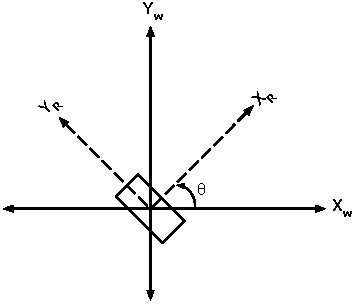
\includegraphics[width = 0.4\linewidth]{Robot_change_of_basis.pdf}
	\caption{\label{robot_ref_frame}World coordinate system and Robot coordinate system}
\end{figure}
%Prob. 10 Extra practice
\item  \Nagy{136}{4.4.4} (Do NOT turn in a solution. No points awarded.) A solution will be provided as extra practice.

%End of list of HW Problems
\end{enumerate}

\newpage

\begin{center}
{\bf Hints}
\end{center}
\noindent \textbf{Hints: Prob. 1} It is not important that $S_1$ and $S_2$ have a finite number of elements. You need to show a double inclusion, namely $$\spanof{S_1 \cup S_2} \subset \spanof{S_1} + \spanof{S_2},~\mbox{and}$$
$$\spanof{S_1} + \spanof{S_2} \subset \spanof{S_1 \cup S_2}.$$
The main thing is to carefully apply the definition of ``span''. What does an element of $\spanof{S_1}$ look like, etc.


\vspace{1cm}

\noindent \textbf{Hints: Prob. 3} Form a general linear combination of the matrices and set it to the zero matrix. Realize that this gives you a set of simultaneous equations for the coefficients you used in your linear combination (due to the matrices being symmetric, you'll get three equations). Now, check if there exists a nontrivial solution to your equations.

\vspace{1cm}


\noindent \textbf{Hints: Prob. 4} If $S_1\subset S_2$, then how is $\spanof{S_1}$ related to $\spanof{S_2}$? What is the span of a subspace?

\vspace{1cm}


\noindent \textbf{Hints: Prob. 5}
\begin{itemize}
\item You need to show that (a) implies (b) and that (b) implies (a). That is what is meant by equivalent.
\item The result is proven in Nagy, Chapter 4. You can copy the proof, using our notation. His vocabulary is slightly different from ours, but that is not important. I am assigning the problem just to force you to read the result and (hopefully) understand it. We'll come back to it in a week or two.
\item What does the uniqueness part mean? It means that if $v_1, v_2 \in V$ and $w_1, w_2 \in W$ are such that $$v_1+w_1 = v_2 + w_2$$
    then $v_1=v_2$ and $w_1=w_2$.
\end{itemize}

\vspace{1cm}

\noindent \textbf{Hints: Prob. 6} Starting from the left and moving to the right, discard a vector if it is linearly dependent on those preceding it. How many vectors remain? The set you obtain is by construction linearly independent and the number of elements is the dimension.

\vspace{1cm}

\noindent \textbf{Hints: Prob. 8} Recall that you can compute whichever of $P$ or $\bar{P}$ is easier, and then, if necessary, invert a matrix in MATLAB to get the final answer.

\vspace{1cm}
\noindent \textbf{Hints: Prob. 9}
\begin{itemize}
	\item Recall coordinate transformations. Since the origins of both coordinate systems coincide, this is a case of pure rotation.
	\item Take any generic point $(x,y)$ and use trigonometry to find the relation between $(x_W,y_W)$ and $(x_R,y_R)$.
\end{itemize}

\end{document}


